\section{Problem Formulation}\label{sec:problem}\label{sec:bench}

\begin{figure*}[!t]
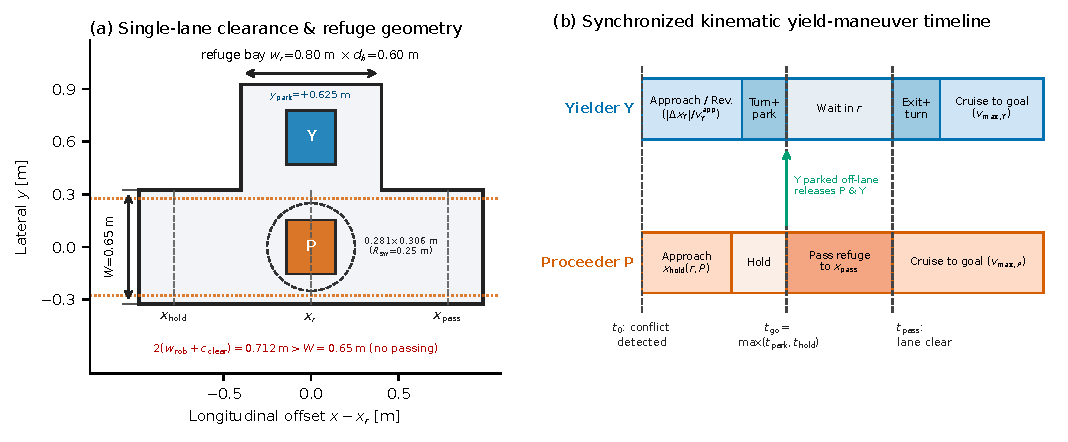
\includegraphics[width=1\textwidth]{Images/problem_formulation.pdf}
\caption{Physical and kinematic formulation of a narrow-corridor encounter. (a) Cross-sectional clearance constraint~\eqref{eq:width_constraint}: two robots of width $w_{\mathrm{rob}}=0.306$\,m with clearance $c_{\mathrm{clear}}=0.05$\,m require $0.712$\,m laterally and cannot pass side by side within corridor width $W=0.65$\,m unless yielder $Y$ parks at lateral offset $y_{\mathrm{park},r}$ inside refuge $r$. (b) Synchronized kinematic yield-maneuver timeline~\eqref{eq:geom}--\eqref{eq:timeline} showing hold point $x_{\mathrm{hold}}(r,P)$, clearance point $x_{\mathrm{pass}}(r,P)$, and phase synchronization instants $t_{\mathrm{park}}$, $t_{\mathrm{go}}$, and $t_{\mathrm{pass}}$.}
\label{fig:formulation}
\end{figure*}

Robots traverse a single-lane corridor too narrow for side-by-side passage; when two travel in opposite directions, one must leave the lane into a discrete refuge. Notation and default parameters are summarized in Supplementary Tables~S-I and S-II.


\subsection{Spatial Domain and Single-Lane Passing Constraint}
A straight corridor of length $L$ and width $W$ along the $x$-axis connects staging rooms at $x \le 0$ and $x \ge L$ (Fig.~\ref{fig:formulation}a). Off-lane refuges $r \in \mathcal{R}$ (pull-in bays and end-room parking spots) have entry coordinate $x_r$, opening width $w_r$, and lateral parking offset $y_{\mathrm{park},r}$.

Robots of width $w_{\mathrm{rob}}$, swept radius $R_{\mathrm{sw}}$, and clearance $c_{\mathrm{clear}}$ track the centerline and cannot pass side by side because

\begin{equation}
2\bigl(w_{\mathrm{rob}} + c_{\mathrm{clear}}\bigr) > W.
\label{eq:width_constraint}
\end{equation}
so one robot must pull into a refuge while the other drives past $x_r$.

\subsection{Robot State and Asymmetric Kinematics}
Robot $i \in \{A, B\}$ has position $x_i$, speed $v_i$, direction $s_i \in \{\pm1\}$, goal $x_{\mathrm{goal},i}$, corridor entry time $t_{\mathrm{enter},i}$, urgency $u_i \ge 1$, and payload flag $l_i \in \{0, 1\}$, and follows unicycle kinematics with acceleration limit $a_{\max,i}$, turn-rate limit $\omega_{\max,i}$, and asymmetric speed limits

\begin{equation}
-v_{\mathrm{rev},i} \le v_i \le v_{\max,i}, \qquad 0 < v_{\mathrm{rev},i} < v_{\max,i}.
\label{eq:speed_bounds}
\end{equation}

Since reversing is slower and entering a bay takes two $90^\circ$ turns, backing into a refuge behind a robot costs far more than pulling into one ahead.

\subsection{Refuge Feasibility Constraints}
When two opposing robots $A$ and $B$ meet, a candidate resolution assigns one robot as the \emph{yielder} $Y \in \{A, B\}$, the other as the \emph{proceeder} $P$, and selects a target refuge $r \in \mathcal{R}$ for $Y$.
For $P$ to pass safely while $Y$ is parked in refuge $r$, three longitudinal coordinates along the centerline govern the maneuver (Fig.~\ref{fig:formulation}a), namely, $P$'s minimum braking coordinate $x_{\mathrm{stop}}$, the hold line $x_{\mathrm{hold}}$ where $P$ must wait if $Y$ is not yet parked, and the clearance line $x_{\mathrm{pass}}$ where $P$ has fully passed the refuge, defined as

\begin{equation}
\begin{aligned}
x_{\mathrm{stop}} &= x_P + s_P \frac{v_P^2}{2 a_{\max,P}}, \\
x_{\mathrm{hold}} &= x_r - s_P \Bigl(\frac{w_r}{2} + R_{\mathrm{sw}} + c_{\mathrm{clear}}\Bigr), \\
x_{\mathrm{pass}} &= x_r + s_P \Bigl(\frac{w_r}{2} + R_{\mathrm{sw}} + c_{\mathrm{clear}}\Bigr).
\end{aligned}
\label{eq:geom}
\end{equation}

A refuge $r \in \mathcal{R}$ belongs to the \emph{feasible refuge set} $\mathcal{F}(Y, P)$ if it is unobstructed and satisfies three conditions along each robot's travel direction, stated below.
\begin{enumerate}
\item \emph{Braking margin:} $P$ can stop before the hold line, $s_P(x_{\mathrm{hold}} - x_{\mathrm{stop}}) \ge 0$;
\item \emph{Proceeder progression:} $P$'s goal lies beyond the clearance line, $s_P(x_{\mathrm{goal},P} - x_{\mathrm{pass}}) \ge 0$; and
\item \emph{Yielder progression:} $Y$'s goal lies beyond the refuge entry, $s_Y(x_{\mathrm{goal},Y} - x_r) \ge 0$.
\end{enumerate}

\subsection{Maneuver Timeline and Delay Model}
Without opposing traffic, robot $i$ cruises directly to its goal in free-flow time $T_i^{\mathrm{free}} = |x_{\mathrm{goal},i} - x_i| / v_{\max,i}$.
When yielder $Y$ pulls into a feasible refuge $r \in \mathcal{F}(Y, P)$, the maneuver unfolds in four sequential stages (Fig.~\ref{fig:formulation}b), summarized below.
\begin{enumerate}
\item \emph{Yielder parks ($t_{\mathrm{park}}$):} $Y$ travels to $x_r$ at speed $v_Y^{\mathrm{app}}$ ($v_{\mathrm{rev},Y}$ if reversing, $v_{\max,Y}$ if driving forward), rotates $90^\circ$ in time $t_{\mathrm{turn}} = (\pi/2)/(0.8\,\omega_{\max,Y})$, and pulls into $y_{\mathrm{park},r}$.
\item \emph{Proceeder holds ($t_{\mathrm{go}}$):} $P$ reaches the hold line at $t_{\mathrm{hold}} = |x_{\mathrm{hold}} - x_P| / v_{\max,P}$ and waits if $Y$ is not yet parked, departing at $t_{\mathrm{go}} = \max(t_{\mathrm{park}},\, t_{\mathrm{hold}})$.
\item \emph{Proceeder passes ($t_{\mathrm{pass}}$):} $P$ drives past the refuge to clear $x_{\mathrm{pass}}$, then continues to $x_{\mathrm{goal},P}$.
\item \emph{Yielder resumes ($T_Y$):} Once $P$ clears $x_{\mathrm{pass}}$, $Y$ reverses out of the bay, rotates $90^\circ$ back onto the centerline, and drives to $x_{\mathrm{goal},Y}$.
\end{enumerate}
The resulting milestone times ($t_{\mathrm{park}}, t_{\mathrm{pass}}$) and total arrival times ($T_Y, T_P$) are given by
\begin{equation}
\begin{aligned}
t_{\mathrm{park}} &= \frac{|x_r - x_Y|}{v_Y^{\mathrm{app}}} + t_{\mathrm{turn}} + \frac{|y_{\mathrm{park},r}|}{v_{\max,Y}}, \\
t_{\mathrm{pass}} &= \max(t_{\mathrm{park}},\, t_{\mathrm{hold}}) + \frac{|x_{\mathrm{pass}} - x_{\mathrm{hold}}|}{v_{\max,P}}, \\
T_Y(r) &= t_{\mathrm{pass}} + \frac{|y_{\mathrm{park},r}|}{v_{\mathrm{rev},Y}} + t_{\mathrm{turn}} + \frac{|x_{\mathrm{goal},Y} - x_r|}{v_{\max,Y}}, \\
T_P(r) &= t_{\mathrm{pass}} + \frac{|x_{\mathrm{goal},P} - x_{\mathrm{pass}}|}{v_{\max,P}}.
\end{aligned}
\label{eq:timeline}
\end{equation}
Each robot's predicted encounter delay is the extra time incurred above free flow, defined as
\begin{equation}
d_i(r) = T_i(r) - T_i^{\mathrm{free}}, \qquad i \in \{Y, P\},
\label{eq:delay_def}
\end{equation}
and the optimal refuge for candidate yielder $Y$ is the feasible refuge that minimizes combined delay, $r^\ast(Y, P) = \arg\min_{r \in \mathcal{F}(Y, P)} [d_Y(r) + d_P(r)]$ (breaking ties by closest $|x_r - x_Y|$).

\subsection{Optimization Objectives and Operational Constraints}
Ideally, when two opposing robots $A$ and $B$ meet with full map knowledge and honest communication, the goal is to choose the yielder $Y \in \{A, B\}$ and feasible refuge $r \in \mathcal{F}(Y, P)$ that minimize total urgency-weighted delay according to
\begin{equation}
\min_{Y \in \{A, B\},\; r \in \mathcal{F}(Y, P)} \; C_{\mathrm{soc}}(Y, r) = u_Y d_Y(r) + u_P d_P(r).
\label{eq:social_obj}
\end{equation}

Without a central controller, solving~\eqref{eq:social_obj} faces the four obstacles behind RQ1--RQ4: robots know their delays only approximately; self-interested robots may misreport them, while cooperative fleets must balance delay across repeated encounters~\cite{jain1984fairness}; messages are lost or delayed and maps are incomplete; and a third robot can block the yielder, while 2D predictions must survive 3D physics and perception.
